In this section we describe our model and compare it to a number of different baseline models. We implement our model as well as the baselines in Python 3.7 using NumPy, Pandas, Scikit-learn and PyTorch. We split the training data into training and test datasets randomly while ensuring that the distributions of human/bot labels in both datasets represent the overall distribution accurately.

We evaluate the model against Gaussian Naïve Bayes (GNB), Quadratic Discriminant Analysis (QDA), a Support Vector Machine (SVM), a $k$-Nearest Neighbors (KNN) and a Random Forest (RF) model. For these baseline models we use the following features:
\begin{align*}
    X_{base} = \{ & \texttt{default\_profile}, \texttt{profile\_image}, \texttt{favourites\_count}, \\
    & \texttt{followers}, \texttt{following}, \texttt{listed\_count}, \texttt{statuses\_count}, \\
    & \texttt{account\_age}, \texttt{reputation} \}
\end{align*}

After evaluating linear, polynomial and RBF kernels for the SVM model, we found the model to perform best with the RBF kernel. The RF model is trained using 100 trees, and splits are performed according to the Gini coefficient. GNB and QDA models are trained using the standard settings in Scikit-learn. 

The neural network classifier is a fully-connected feedforward neural network. After much experimentation we chose to use 3 hidden layers with $(500, 200, 100)$ neurons respectively, using batch normalization and dropout with $p=0.5$. The model is trained using Adam and a learning rate of $\eta = 0.001$ for 750 epochs. We find that the model achieves better performance and generalizes better when we remove outliers that deviate from the mean by more than three standard deviations from the training dataset.

We experimented with different sets of features and found a set of neighborhood features (NF) and graph features (GF) described in section \ref{sec:approach} that performs best along with the baseline features. We also found that removing some of the original features along with adding the  NF and GF improved the performance of our classification model. The final set of features used in our classifier are:
\begin{alignat*}{2}
    & X_{NF} = \{ && \texttt{favourites\_count}, \texttt{statuses\_count}, \texttt{outdegree\_predecessors}, \\
    & && \texttt{favorites\_predecessors}, \texttt{status\_predecessors}, \\
    & && \texttt{age\_predecessors}, \texttt{account\_age}, \texttt{following}, \texttt{followers} \} \\
    \\
    & X_{GF} = && \{ \texttt{ego\_density}, \texttt{ego\_reciprocity} \}
\end{alignat*}

\begin{table}[t]
\centering
\setlength{\tabcolsep}{12pt}
\begin{tabular}{@{}lccccc@{}}
\toprule
\textbf{Model} & \textbf{Accuracy} & \textbf{TPR} & \textbf{FPR} & \textbf{F1 score} & \textbf{AUC} \\ \midrule
GNB             & 0.6399 & \textbf{0.9622} & 0.7313 & 0.741  & 0.6154 \\
QDA             & 0.6751 & 0.8937 & 0.5768 & 0.7465 & 0.6584 \\
SVM             & 0.7797 & 0.7746 & 0.2145 & 0.7901 & 0.7801 \\
KNN             & 0.8496 & 0.8752 & 0.18   & 0.8617 & 0.8476 \\
RF              & 0.8675 & 0.8745 & 0.1405 & 0.876  & 0.867 \\
NN              & 0.8648 & 0.8673 & 0.138  & 0.8729 & 0.8646 \\ \midrule
NN + NF (ours)  & 0.8702 & 0.8623 & \textbf{0.1208} & 0.8767 & 0.8708 \\
NN + NF + GF (ours) & 0.8732 & 0.883 & 0.138 & 0.8818 & 0.8725 \\
RF + NF + GF (ours) & \textbf{0.8774} & 0.888 & 0.1348 & \textbf{0.8858} & \textbf{0.8766} \\
\bottomrule
\end{tabular}
\caption{Results on the \textsc{Cresci-2018} dataset for various baseline models (top) and our model using neighborhood features (bottom).}
\label{tab:results}
\end{table}

\noindent We denote the number of correctly positively classified samples as TPR (true-positive rate) whereas FPR is the number of falsely positively classified samples (false-positive rate). The models are evaluated in terms of:
\begin{itemize}
    \item[1.] Accuracy
    \item[2.] TPR
    \item[3.] FPR
    \item[4.] F1 score
    \item[5.] area under the ROC curve (AUC)
\end{itemize}

Our model outperforms the baseline models on the \textsc{Cresci-2018} dataset (table~\ref{tab:results}). We notice that both the GNB and QDA model are not very good at identifying bot accounts on this dataset accurately and have a very high false positive rate. The SVM model is slightly better and achieves an F1 score of 0.79. Interestingly, KNN is surprisingly effective on this dataset and only slightly less effective than the RF and NN models. Both RF and NN turn out to be very effective and achieve the highest scores. Due to this, we chose to focus only on the RF and NN models for our proposed extensions and sets of features. By using the proposed NF we see an overall improvement both for the RF and NN models.

It is interesting to note that actually only a set of certain, very few features is sufficient to effectively separate bots and humans in multi-dimensional space. We find that the number of a user's favourites, followers and statuses actually suffice to identify very clear differences in the distribution of human and bot accounts (figure \ref{fig:3dvis}). Indeed, a RF classifier is able to achieve an F1 score of 0.8781 and AUC of 0.8705 using only those three features and actually performs better than all of the baseline models which were trained on all features retrieved using the Twitter API.

\begin{figure}
    \centering
    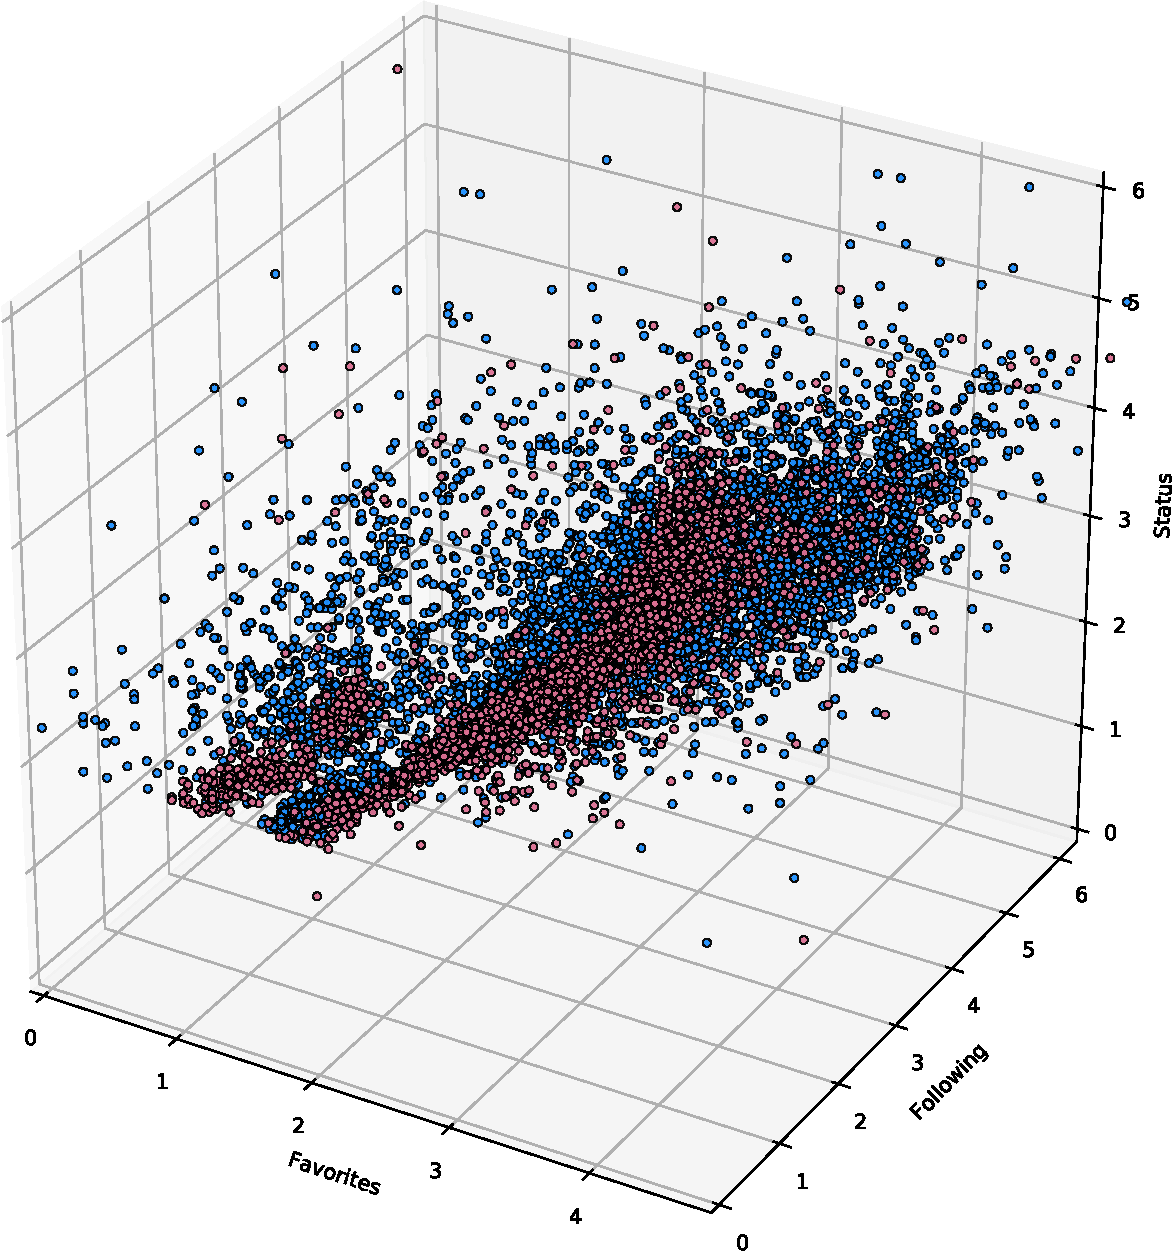
\includegraphics[width=0.6\textwidth]{paper/FIG/3dvis_base-crop.pdf}
    \caption{We can clearly see the different distributions of humans (blue) and bots (red). All axes are plotted in log scale.}
    \label{fig:3dvis}
\end{figure}

Lastly, we would like to note the fact that \textsc{Cresci-2018} may not have been the ideal dataset and we believe that this method could work much better on higher quality data and particularly well for data with bots who deviate stronger from the norm in terms of social structure in the graph. This dataset was collected from so called ``stock Twitter'', a subset of Twitter users that mainly talk about stocks and market movements, and the data was focused on bots that aim to influence the market by shaping the perception of public opinion on Twitter through retweeting (i.e. sharing with their followers) of suspicious ``peak tweets''~\cite{cresci2018fake}. We have noticed that this is also reflected in the users contained in the datasets and that these users may not be easily and reliably identified using only profile, and graph neighborhood data. Additionally, many users in the dataset that are labelled as bots do not immediately strike us as bots upon manual review which brings the quality of the dataset into question. In general the in- and out-degrees of users in the dataset (for both human and bot accounts) seem much higher than we would expect from a random sample of Twitter users. Despite these circumstances we find that our approach works and is able to improve upon baseline classification models for ``free": it does not require any additional labelled data and simply augments existing labelled data by use of data from neighbors in the social graph. 